\documentclass{article}

\usepackage{graphicx}

\begin{document}

\section{Introduction}\label{introduction}

\subsection{What is the purpose of a
spectrometer?}\label{what-is-the-purpose-of-a-spectrometer}

A \emph{spectrometer} is used to record and measure the spectral content
of signals, such as radio waves received from astronomical sources.
Analysis of the spectral content can reveal details of the radio sources
themselves as well as properties of the intervening medium.
Spectrometers can increase the signal to noise ratio (SNR) of a radio
telescope through both integration and channelization.

Integration increases the SNR because signal increases linearly with
integration whereas noise increases as the square root with integration.
Thus, integrating longer by a factor of N will increase SNR by a factor
of sqrt(N).

Channelization reduces the signal to noise of narrowband signals due to
the fact that the noise power is divided equally across all spectral
channels while the narrow band signal is confined to a comparatively
smaller number of channels. For a sinusoidal signals, channelizing to N
channels will reduce the per-channel noise power by a factor of N
thereby increasing the per-channel SNR by a factor of N.

\section{Spectrometer Technologies}\label{spectrometer-technologies}

Spectrometers can be created in a number of ways. Most involve multiple
measurements of narrow bands of the original signal, but some are more
esoteric such as acousto-optic spectrometers.

\subsection{Swept Spectrometer}\label{swept-spectrometer}

A \emph{swept spectrometer} uses a variable oscillator with a heterodyne
circuit and a low pass filter. The oscillator is typically varied,
i.e.~swept, through a range of desired frequencies. As it is swept
through the desired frequency range, the power of the low pass filter's
output is measured and recorded. Most analog spectrum analyzers operate
in this manner.

\subsection{Analog Filter Bank}\label{analog-filter-bank}

An \emph{analog filter bank} is just what it's name implies: a bank (or
collection) of analog filters. The analog filters are designed to pass
through different ranges of frequencies. The power of the analog
filters' output is measured and recorded. By creating a bank of filters
with adjacent and non-overlapping passband frequencies one can get a
complete picture of the input signal's spectrum.

\subsection{Autocorrelators}\label{autocorrelators}
The power spectrum of a signal, $S(f)$,  is related to the signal's autocorrelation function, $R(\tau)$, over a range of time lags, $\tau$, by Fourier transform:
\begin{equation}
\label{spec-from-autocorr}
 S(f) = \int_{-\infty}^{\infty} R(\tau)e^{-2\pi i \tau f} \,\mathrm{d}\tau \,.
\end{equation}

Thus, if one can build a device to measure the autocorrelation function of a signal of interest, it is straightforward to obtain the signal's power spectrum.
When integrated over a time $T$, the autocorrelation of a signal specified by the time-varying voltage $v(t)$ is defined by 

\begin{equation}
\label{autocorr}
 R(\tau) = \frac{1}{2T} \int_{-T}^{T} v(t)v(t+\tau) \,\mathrm{d}t \,.
\end{equation}

Since $v(t)$ is a real-valued function $R(\tau)$ is necessarily symmetric about positive and negative lags, so only one half need be measured. Furthermore, the symmetry of $R(\tau)$ means that the only contributions to $S(f)$ are from the even parts of the complex exponential in Equation \ref{spec-from-autocorr}. The computation of the power spectrum can then be reduced to:

\begin{equation}
\label{spec-from-autocorr-reduced}
 S(f) = 2\int_{0}^{\infty} R(\tau)\cos{(2\pi \tau f)} \,\mathrm{d}\tau \,.
\end{equation}

Regardless of autocorrelator implementation, it is invariably the case that Equation \ref{spec-from-autocorr-reduced} is computed for only a discrete range of delays, $\tau$. In much the same way as the sampling rate of an analog signal determines how much bandwidth can be processed unambiguously (see Section \ref{analog-to-digital-converters}) the spacing of lags in an autocorrelator determines how much bandwidth it can process without aliasing occuring. In the case of an autocorrelator the Nyquist criterion is satisfied when there are two taps per wave period at the highest frequency (shortest wavelength) signal of interest. 


\subsubsection{Analog Autocorrelators}\label{analog-autocorrelators}

Analog correlators are those that measure the autocorrelation function (Equation \ref{autocorr}) using analog circuitry to implement multipliers and propagation times through carefully constructed delay lines to implement the desired tap delays.
A typical schematic of an analog autocorrelator is shown in Figure \ref{fig:analog-autocorr}. Here, outputs of each correlator tap are digitized after a small amount of time-averaging. Further averaging can take place digitally before computation of the power spectrum via cosine transform. Details of specific scientific deployments of analog autocorrelation spectrometers can be found in \cite{Erickson2007} and \cite{Harris1998}.

The main advantage of the analog autocorrelator over its digital counterpart (see Section \ref{digital-autocorrelators}) is that digitization need only take place at a rate commensurate with the averaging period of the correlator, rather than the bandwidth of the input signals. For this reason, analog autocorrelation spectrometers are usually seen in systems that have instantaneous bandwidths of many gigahertz which cannot be readily digitized by commercially available ADCs.


\begin{figure}
 \centering
 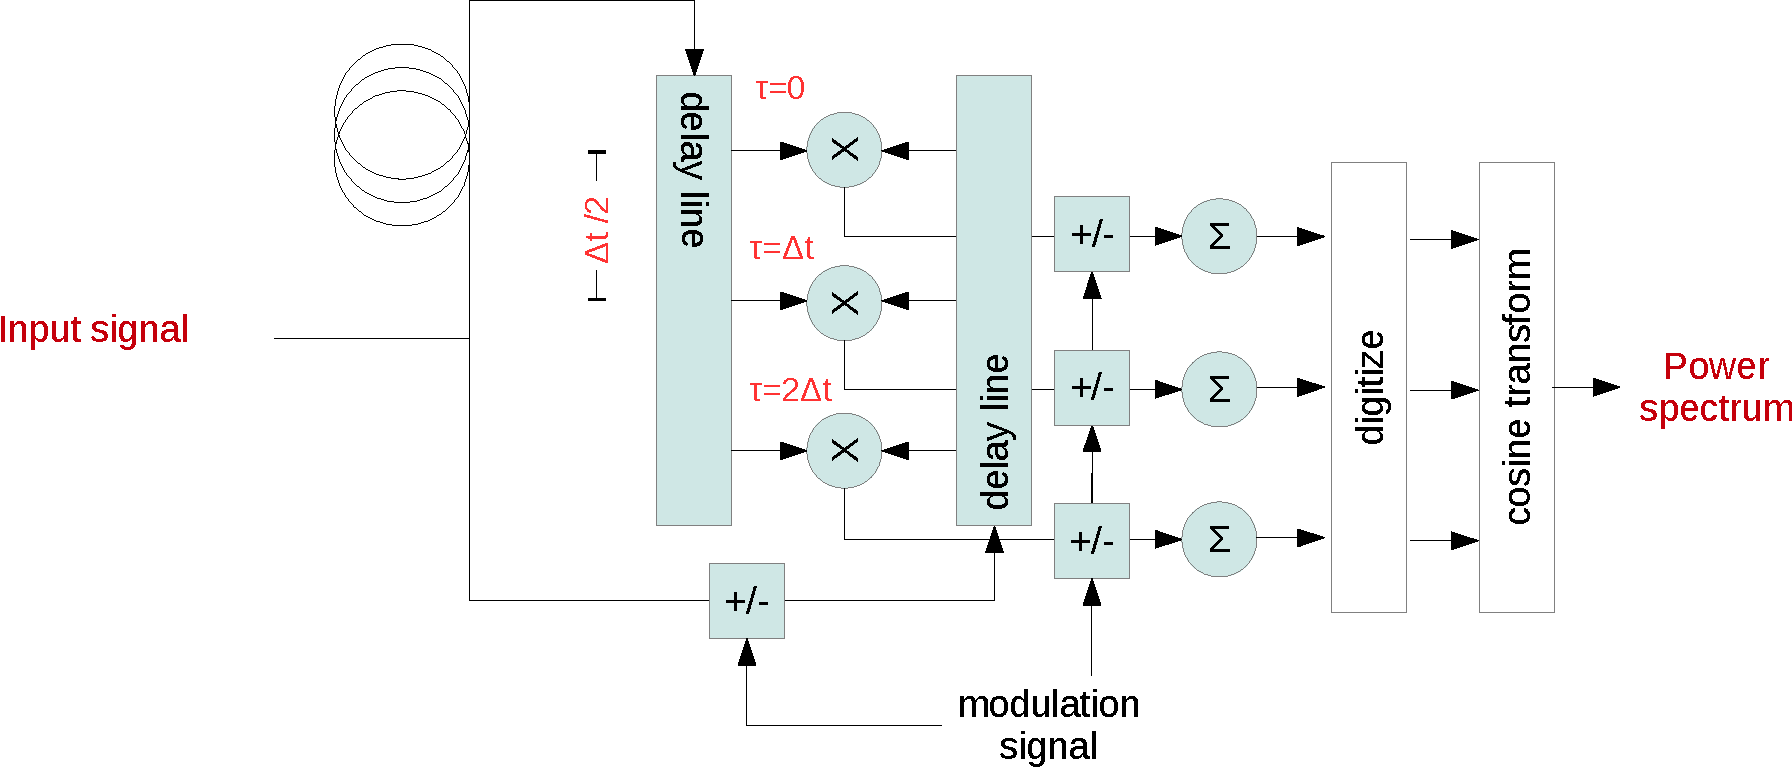
\includegraphics[width=\textwidth]{./figures/analog-autocorr-crop.pdf}
 % analog-autocorr-crop.pdf: 0x0 pixel, 0dpi, nanxnan cm, bb=
 \label{fig:analog-autocorr}
 \caption{An example implementation of an analog autocorrelator. The input signal is circulated in opposite directions down a pair of delay lines. The signal is tapped on each delay line at points separated by propagation delays of $\frac{\Delta t}{2}$. Each tap computes an element of the correlation with lag $\tau=n\Delta t$.}
\end{figure}

Figure \ref{fig:analog-autocorr} also indicates circuitry for modulating the input and outputs of the correlator. Such switching can serve multiple purposes. Firstly, it is sometimes advantageous for cost or performance reasons to prefer square-law diode detectors in favour of multiplication circuitry. These have a respose to inputs $v_1$ and $v_2$ of
\begin{equation}
 v_1^2 + v_2^2 + 2v_1v_2 \, .
\end{equation}

The last term is equal to the output of a multiplier, while the first two terms represent unwanted parts of the diode response. These unwanted terms can be eliminated by periodically alternating the sign of one of the inputs $v_1$ or $v_2$. This has no effect on the unwanted terms, but causes the last term to alternate sign. If, prior to time averaging, the sign of the diode output is flipped synchronously with the input then the unwanted terms will, up to a noise contribution, be removed.

In general, the principal of modulating the desired part of a signal and then synchronously demodulating to cancel out unwanted contributions can be used to surpress a variety of unwanted effects in radio receivers, such as gain variation and cross-coupling. An operating telescope may have multiple such switching systems operating concurrantly at different frequencies targetting different effects. See, for example, \cite{Erickson2007}. 


\subsubsection{Digital Autocorrelators}\label{digital-autocorrelators}
Digital autocorrelators implement the autocorrelators delay-and-multiply circuitry using digital delays -- shift registers -- and digital multiplier cores to compute signal products. As a result, digital correlators can have much more predictable performance than their analog counterparts whose processing is subject to small errors in delay line lengths and other subtle analog effects. In contrast, provided signals in a digital autocorrelator can be digitised with adequate signal-to-noise and linearity the downstream autocorrelation computation can be regarded as possesing perfect precision.

Digital systems are usually prefered when the bandwidth to be processed is within the capabilities of commercially available ADC chips. However, if the number of frequency channels desired is large an FFT-based spectrometer may be preferable to an autocorrelation system. FFT spectrometers are described more fully in Section \ref{digital-fft} and can be inplemented with vastly lower computational overhead, at the cost of increased design complexity.

\subsection{Acousto-Optic}\label{acousto-optic}

\subsection{Hybrid Analog-Digital}\label{hybrid-analog-digital}

\subsection{Digital FFT}\label{digital-fft}

\section{Analog to Digital
Converters}\label{analog-to-digital-converters}

As their name implies, \emph{analog to digital converters} (ADCs)
convert analog signals into digital signals. The two main
characteristics of an ADC are its sample rate and tbe number of bits per
sample.

The ADC converts an analog voltage into a numeric quantity and then
repeats the process. The numeric quantities are called \emph{samples}.
The rate at which the ADC performs conversions is called the
\emph{sample rate}. The sample rate, usually expressed in samples per
second, determines the amount of bandwidth that can be unambiguoysly
processed by an ADC. The Nyquist Theorem states that a band limited
signal can be fully recovered when it is sampled at a rate that is twice
the bandwidth. For example, a sample rate of 1 billion s

%% What's Available Commercially

%% Number of Bits vs SNR Loss

%% Van Vleck and Non-Linearities

%% Number of Bits Required for RFI/Strong Signals

%% Interleaving

%% Breaking up a Large Bandwidth into Sub-Bands

% Digital FFT Based Spectrometers

%% Block diagram

%% Polyphase Filter Banks

%% Stokes Parameters

%% Technologies:

    * GPU
    * CPU
    * ASIC
    * FPGA
    * Heterogeneous

% CASPER spectrometers

%% Intro to CASPER

%% Open Source Gateware, GPUware, Software

%% Open Source ADC's and FPGA Boards

%% Multi-Purpose Radio Astronomy Instrumentation

%% Fast Readout Spectrometers for Pulsar Timing and Search

%% Multibeam Spectrometer Synchronization

\bibliographystyle{plain}
\bibliography{spectrometers}

%\bibliography{spectrometers.bib}

\end{document}
